\section{Стохастический анализ}

    \subsection{Описание изменений}

        Пришло время провести стохастический анализ. В модели появляется слагаемое, которое отвечает за шум. Это слагаемое имеет следующий вид: \(\varepsilon \xi\), где \(\varepsilon\) --- интенсивность шума, а \(\xi\) --- нормальная случайная величина.

        В данную модель шум можно внести тремя способами.

        \(\alpha\)-шум: 

        \[
            x_{t + 1} = \frac{(\alpha + \varepsilon \xi) x_t^2}{(\beta + x_t)^6}
        \]

        \(\beta\)-шум:

        \[
            x_{t + 1} = \frac{\alpha x_t^2}{(\beta + \varepsilon \xi + x_t)^6}
        \]

        Аддитивный шум:

        \[
            x_{t + 1} = \frac{\alpha x_t^2}{(\beta + x_t)^6} + \varepsilon \xi
        \]

    \subsection{Временные ряды}

        С помощью временных рядов продемонстрируем как различные виды шума влияют на поведение системы.

        \begin{figure}
            \centering
            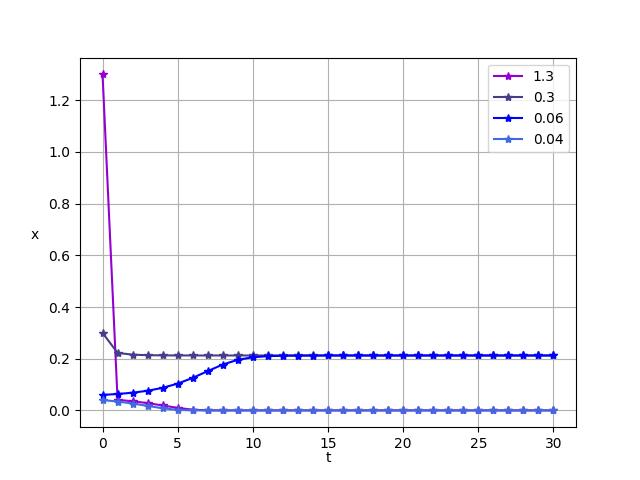
\includegraphics[width=\textwidth]{time_series_b_0_56.jpg}

            \captionsetup{justification=centering}
            \caption{Временные ряды модели (\ref{origin}) для \(\beta = 0.56\) при различных начальных значениях}
            \label{time_series_b_0_56}
        \end{figure}
